%
% Module 5 Chapter 9 Program Documentation
% CSC160-C00: Computer Science I (C++) (Jeffrey Hemmes)
% Author: Ashton Hellwig
% Date: 02 April 2020
%


\documentclass[a4paper, 11pt]{article}
  % Packages
  \usepackage[utf8]{inputenc}         % Encoding
  \usepackage[english]{babel}         % Internationalization
  \usepackage{times}                  % Times New Roman font
  \usepackage{soul}                   % Highlighting
  \usepackage{hyperref}               % Links (internal and external)
  \usepackage{fancyhdr}               % Headers and footers
  \usepackage[dvipsnames]{xcolor}     % Text Colors
  \usepackage{listings}               % Code Snippets
  \usepackage[section]{algorithm}     % For TOC support
  \usepackage{algpseudocode}          % Algorithmic notation environments
  \usepackage{enumitem}               % Ordered lists
  \usepackage{geometry}               % Page layout
  \usepackage{graphicx}               % Image support
  \usepackage{wrapfig}                % Sideways figures (landscape)
  \usepackage{lscape}                 % Sideways figures (landscape)
  \usepackage{rotating}               % Sideways figures (landscape)
  \usepackage{epstopdf}               % Sideways figures (landscape)
  \usepackage[toc, page]{appendix}    % Appendix
  \usepackage{setspace}               % Paragraph and line spacing
  \usepackage{bookmark}               % Required for appendix
  \usepackage{adjustbox}              % Required for appendix
  \usepackage{csquotes}               % Required for appendix
  \usepackage{amsthm}                 % Theorem environments
  \usepackage{array}                  % Arrays
  \usepackage{makecell}               % Table helpers
  \usepackage{amsmath}                % Mathematical symbols
  \usepackage[fleqn]{mathtools}       % Mathematical environments
  \usepackage{amssymb}                % Misc. symbols for logic and math
  \usepackage{relsize}                % Relative Sizing
  \usepackage{multicol}               % Multi-figure displays (grid)
  \usepackage{etoolbox,refcount}      % Required for mdframed
  \usepackage{parcolumns}             % Paragraph grids
  \usepackage{mdframed}               % Colored box environments
  \usepackage{float}                  % Floating Environments 
  \usepackage{aliascnt}               %
  \usepackage{multirow}               % Multiple rows in tables
  \usepackage[                        % Bibliography management
    backend=biber,%
    style=apa%
  ]{biblatex}

  % Bibliography Setup
  \addbibresource{main.bib}
  \DeclareBibliographyCategory{consulted}
  \addtocategory{consulted}{textbook}
  % \newcommand{\CiteSection}[2]{%
    % (\autocite{#1}, ~\S {#1})%
  % }

%   \UseRawInputEncoding

  % Tables
  \renewcommand\theadalign{bc}
  \renewcommand\theadfont{\bfseries}
  \renewcommand\theadgape{\Gape[4pt]}
  \renewcommand\cellgape{\Gape[4pt]}

  % Lists
  \newcounter{countitems}
  \newcounter{nextitemizecount}
  \newcommand{\setupcountitems}{%
    \stepcounter{nextitemizecount}%
    \setcounter{countitems}{0}%
    \preto\item{\stepcounter{countitems}}%
  }
  \makeatletter
  \newcommand{\computecountitems}{%
    \edef\@currentlabel{\number\c@countitems}%
    \label{countitems@\number\numexpr\value{nextitemizecount}-1\relax}%
  }
  \newcommand{\nextitemizecount}{%
    \getrefnumber{countitems@\number\c@nextitemizecount}%
  }
  \newcommand{\previtemizecount}{%
    \getrefnumber{countitems@\number\numexpr\value{nextitemizecount}-1\relax}%
  }
  \makeatother
  \newenvironment{AutoMultiColItemize}{%
  \ifnumcomp{\nextitemizecount}{>}{3}{\begin{multicols}{2}}{}%
  \setupcountitems\begin{itemize}}%
  {\end{itemize}%
  \unskip\computecountitems\ifnumcomp{\previtemizecount}{>}{3}{\end{multicols}}{}}


  % Theorems
  \theoremstyle{definition}
  \newtheorem{defn*}{Definition}
  \theoremstyle{plain}
  \newtheorem{theorem*}{Equation}

  % Colors
  \newcommand{\commentstylecolor}{\color{Gray}}
  \newcommand{\keywordstylecolor}{\color{MidnightBlue}}
  \newcommand{\stringstylecolor}{\color{ForestGreen}}
  \newcommand{\questioninput}{\color{Red}}
  \newcommand{\answertcolor}{\color{Green}}
  \newcommand{\myanswer}{\answertcolor{\hl}}

  % Symbols
  \newcommand{\answerflow}{\rotatebox[origin=c]{180}{$\Lsh$}}
  \newcommand{\toanswer}{\mathlarger{\mathlarger{\answerflow}}\quad}

  % Math
  \newcommand{\highlight}[1]{%
    \colorbox{green!50}{$\displaystyle#1$}}

  % Image Directory
  \graphicspath{ {screenshots/} }


  % Hyperlink Setup
  \hypersetup{
    colorlinks = true,
    urlcolor = blue,
    linkcolor = blue
  }


  % Algorithm Settings
  \newcommand{\pluseq}{\mathrel{{+}{=}}}
  \newcommand{\minuseq}{\mathrel{{-}{=}}}


  % Syntax-Highlighting for Code Snippets
  \lstset{
    backgroundcolor=\color{white},
    breaklines=true,%
    captionpos=b,%
    frame=tlrb,%
    tabsize=2,%
    numbers=left,%
    showstringspaces=false,%
    commentstyle=\commentstylecolor,%
    keywordstyle=\keywordstylecolor,%
    stringstyle=\stringstylecolor%
  }
  \lstset{literate=
  {á}{{\'a}}1 {é}{{\'e}}1 {í}{{\'i}}1 {ó}{{\'o}}1 {ú}{{\'u}}1
  {Á}{{\'A}}1 {É}{{\'E}}1 {Í}{{\'I}}1 {Ó}{{\'O}}1 {Ú}{{\'U}}1
  {à}{{\`a}}1 {è}{{\`e}}1 {ì}{{\`i}}1 {ò}{{\`o}}1 {ù}{{\`u}}1
  {À}{{\`A}}1 {È}{{\'E}}1 {Ì}{{\`I}}1 {Ò}{{\`O}}1 {Ù}{{\`U}}1
  {ä}{{\"a}}1 {ë}{{\"e}}1 {ï}{{\"i}}1 {ö}{{\"o}}1 {ü}{{\"u}}1
  {Ä}{{\"A}}1 {Ë}{{\"E}}1 {Ï}{{\"I}}1 {Ö}{{\"O}}1 {Ü}{{\"U}}1
  {â}{{\^a}}1 {ê}{{\^e}}1 {î}{{\^i}}1 {ô}{{\^o}}1 {û}{{\^u}}1
  {Â}{{\^A}}1 {Ê}{{\^E}}1 {Î}{{\^I}}1 {Ô}{{\^O}}1 {Û}{{\^U}}1
  {œ}{{\oe}}1 {Œ}{{\OE}}1 {æ}{{\ae}}1 {Æ}{{\AE}}1 {ß}{{\ss}}1
  {ű}{{\H{u}}}1 {Ű}{{\H{U}}}1 {ő}{{\H{o}}}1 {Ő}{{\H{O}}}1
  {ç}{{\c c}}1 {Ç}{{\c C}}1 {ø}{{\o}}1 {å}{{\r a}}1 {Å}{{\r A}}1
  {€}{{\euro}}1 {£}{{\pounds}}1 {«}{{\guillemotleft}}1
  {»}{{\guillemotright}}1 {ñ}{{\~n}}1 {Ñ}{{\~N}}1 {¿}{{?`}}1
}
  \newenvironment{alltt}{\ttfamily}{\par}
  \lstMakeShortInline[language=c++,columns=fixed]|

  % Page Configuration
  %% Style
  \pagestyle{fancy}

  %% Layout
  \geometry{%
    a4paper,%
    top=2.5cm,%
    bottom=2.5cm,%
    left=2.5cm,%
    right=2.5cm%
  }
  %%% Document
  \setlength{\headheight}{15pt}
  \setlength{\floatsep}{12pt}
  \setlength{\parindent}{2em}
  \setlength{\parskip}{0.5em}
  \renewcommand{\baselinestretch}{.9}

  %% Title page
  \title{Chapter 9 Programming Assignment Documentation}
  \author{Ashton Hellwig}
  \date\today
  \setcounter{tocdepth}{3}

  %% Subsequent pages
  \lhead{CSC160}
  \rhead{Computer Science I (C++)}
  \lfoot{M4C8Program}
  \rfoot{A. Hellwig}


  % Document Content
\begin{document}
  % Title Page
  \maketitle
  \tableofcontents
  \listofalgorithms
  \lstlistoflistings
  \newpage


  % Problem Analysis
  \section{Problem Analysis}
    The problem states:
    \begin{mdframed}[backgroundcolor=green!20]
      This assignment relates to content from Chapter 9 of the eText.

      \textbf{Instructions}\vspace{-8pt}
      \begin{enumerate}
        \item Review the general programming assignment instructions.
        \item Write a program that:
          \begin{enumerate}[label=\Alph*.]
            \item Allows the user to enter the last names of five candidates in
              a local election and the number of votes received by each candidate.
            \item The program should then output each candidate’s name, the
              number of votes received, and the percentage of the total votes
              received by the candidate.
            \item Your program should also output the winner of the election.
            \item This program must be done using parallel arrays to store the
              name and number of votes for each candidate.
            \item The number must be formatted appropriately as shown in the
              sample output below.
          \end{enumerate}
      \end{enumerate}
    \end{mdframed}

    \subsection{Data}
      \begin{itemize}
        \item We need two parallel arrays which should match index$\rightarrow$%
          index.
          \begin{itemize}
            \item |std::string candidateLastName[];| to store the candidate's
              name.
            \item |int candidateVotes[];| to store the number of votes received
              by the candidate.
          \end{itemize}
      \end{itemize}

    \subsection{Desired Output}
      \begin{lstlisting}[%
        language=bash,%
        columns=flexible,%
        caption={ashellwig\_m5c9\_programming\_assignment output %
          (stdout)},%
        label={desiredoutput:stdout}%
    ]
Enter candidates name and the votes received by the candidate.
Smith 12345
Jones 4567
Adams 555
Washington 888888
Jefferson 456789
Candidate    Votes Received    % of Total Votes
Smith           12345               0.91
Jones            4567               0.34
Adams             555               0.04
Washington     888888              65.21
Jefferson      456789              33.51
Total            1363144
The Winner of the Election is Washington
Press any key to continue...
  \end{lstlisting}


  % Algorithm
  \newpage
  \section{Algorithm}
    Below is the algorithm for the program.

    % !TEX root = ../main.tex
%
% Module 5 Chapter 9 Program Algorithm
% CSC160-C00: Computer Science I (C++) (Jeffrey Hemmes)
% Author: Ashton Hellwig
% Date: 02 April 2020
%


\begin{algorithm}[H]
    \caption{Chapter 9 Program Algorithm}
    \vspace{12pt}
    \begin{algorithmic}[1]
      \Procedure{main}{}
        \State\Return $0$
      \EndProcedure
    \end{algorithmic}
    \label{alg}
  \end{algorithm}
 


  % User Documentation
  \newpage
  \section{User Documentation}
    Please see Appendix \ref{appendix:img} for images showing the compilation
      and running of the program.

    %% Usage
    \subsection{Build}
      The following are instructions with two use cases:
      \begin{itemize}
        \item With GNU Make
        \item Bundled Release
      \end{itemize}
      \subsubsection{With GNU Make}
        \begin{enumerate}
          \item Navigate to the unzipped folder containing the project,
            \textbf{with a terminal emulator or command prompt}, this will
            (most likely) mean running:
            \begin{lstlisting}[language=bash]
cd ~/Downloads/ashellwig_m5c9_programming_assignment
            \end{lstlisting}
          \item Compile the program and documentation\footnote{\textbf{Note%
            }: This requires the whole \texttt{texlive} suite as well as
            \texttt{latexmk} to be installed.} using GNU automake after
            switching to the source directory:
            \begin{lstlisting}[%
              language=bash,%
              caption={Chapter 9 Program Build Commands},%
            ]
make debug

./out/bin/ashellwig_m5c9_programming_assignment.bin # Run program

make clean-all # Removes object files, binaries, and docs
            \end{lstlisting}
          \end{enumerate}
      \subsubsection{Bundled Release}
        \begin{enumerate}
          \item Navigate to the unzipped folder containing the binary,
            \textbf{with a terminal emulator or command prompt}, this will
            (most likely) mean running:
            \begin{lstlisting}[language=bash]
cd ~/Downloads/ashellwig_m5c9_programming_assignment/out/bin
            \end{lstlisting}
          \item To run the program simply issue this within the command
            prompt
            \begin{lstlisting}[language=bash]
./build/ashellwig_m5c9_programming_assignment
            \end{lstlisting}
        \end{enumerate}
        Of course if preferred, you may also navigate to the build folder in
          file explorer and double click the executable
          (\texttt{./ashellwig\_m5c9\_programming\_assignment}).


  % Bibliography
  \newpage
  \nocite{*}
  % \printbibliography[%
  %   heading=bibintoc,%
  %   title={Works Cited},%
  %   notcategory={consulted}%
  % ]{}
  \printbibliography[%
    heading=bibintoc,%
    title={Works Consulted},%
    category={consulted}%
  ]{}

  % Appendix
  \appendix
  \newpage
  % Images
  \section{Images}\label{appendix:img}
    \begin{figure}[H]
      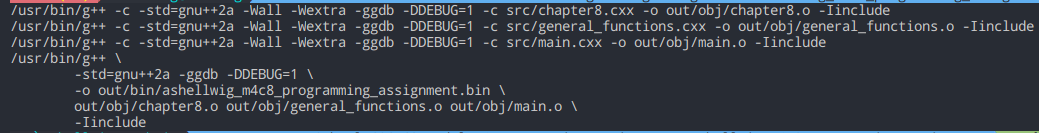
\includegraphics[%
        width={\textwidth}%
      ]{compile.png}
      \caption{Compiling Chapter 9`s Program}
      \label{img:compilation}
    \end{figure}
    \begin{figure}[H]
      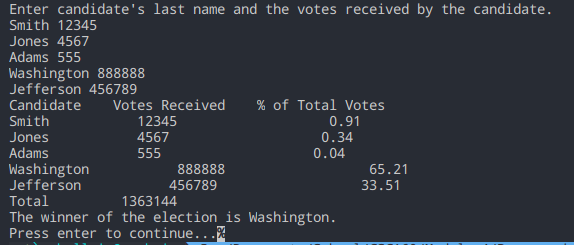
\includegraphics[%
        width=\textwidth%
      ]{run.png}
      \caption{Running Chapter 9`s Program}
      \label{img:running}
    \end{figure}


  \newpage
  \section{Unit Tests}
    Tests were written with the
      \href{https://github.com/catchorg/catch}{Catch2 library}. The output is
      shown below.

    \begin{figure}[H]
      \caption{Test Output}
      \centering
      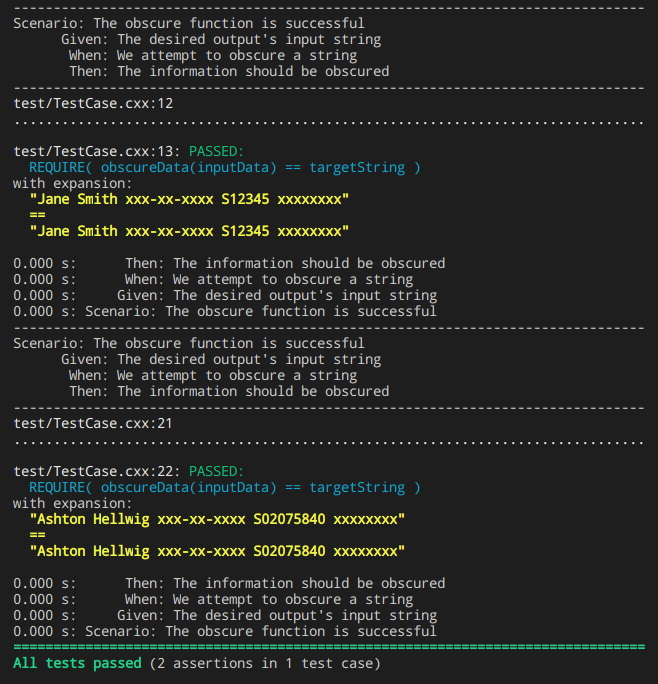
\includegraphics[width=\textwidth]{testout.png}
    \end{figure}

    \newpage
    \subsection{Unit Test File}
      Below I have included the code used to run the unit test for reference.

      \begin{lstlisting}[language=c++,caption={TestCase.cxx}]
#include "../include/catch2/catch.hpp"
      \end{lstlisting}
\end{document}

